%&latex
%&latex
\documentclass[namedreferences]{SolarPhysics}
\usepackage[optionalrh,solaenum]{spr-sola-addons} % For Solar Physics 
%\usepackage{epsfig}          % For eps figures, old commands
\usepackage{graphicx}        % For eps figures, newer & more powerfull
%\usepackage{courier}         % Change the \texttt command to courier style
%\usepackage{natbib}         % For citations: redefine \cite commands
%\usepackage{amssymb}        % useful mathematical symbols
\usepackage{color}           % For color text: \color command
\usepackage{url}             % For breaking URLs easily trough lines
\def\UrlFont{\sf}            % define the fonts for the URLs


% General definitions
% please place your own definitions here and don't use \def but
% \newcommand{}{} or 
% \renewcommand{}{} if it is already defined in LaTeX

\newcommand{\BibTeX}{\textsc{Bib}\TeX}
\newcommand{\etal}{{\it et al.}}

% Definitions for equations
\newcommand{\deriv}[2]{\frac{{\mathrm d} #1}{{\mathrm d} #2}}
\newcommand{\rmd}{ {\ \mathrm d} }
\renewcommand{\vec}[1]{ {\mathbf #1} }
\newcommand{\uvec}[1]{ \hat{\mathbf #1} }
\newcommand{\pder}[2]{ \f{\partial #1}{\partial #2} }
\newcommand{\grad}{ {\bf \nabla } }
\newcommand{\curl}{ {\bf \nabla} \times}
\newcommand{\vol}{ {\mathcal V} }
\newcommand{\bndry}{ {\mathcal S} }
\newcommand{\dv}{~{\mathrm d}^3 x}
\newcommand{\da}{~{\mathrm d}^2 x}
\newcommand{\dl}{~{\mathrm d} l}
\newcommand{\dt}{~{\mathrm d}t}
\newcommand{\intv}{\int_{\vol}^{}}
\newcommand{\inta}{\int_{\bndry}^{}}
\newcommand{\avec}{ \vec A}
\newcommand{\ap}{ \vec A_p}
\newcommand{\bb}{ \vec B}
\newcommand{\jj}{ \vec j}
\newcommand{\rr}{ \vec r}
\newcommand{\xx}{ \vec x}

% Definitions for the journal names
\newcommand{\adv}{    {\it Adv. Space Res.}}
\newcommand{\annG}{   {\it Annales Geophysicae}}
\newcommand{\aap}{    {\it Astron. Astrophys.}}
\newcommand{\aaps}{   {\it Astron. Astrophys. Suppl.}}
\newcommand{\aapr}{   {\it Astron. Astrophys. Rev.}}
\newcommand{\ag}{     {\it Ann. Geophys.}}
\newcommand{\aj}{     {\it Astron. J.}}
\newcommand{\apj}{    {\it Astrophys. J.}}
\newcommand{\apss}{   {\it Astrophys. Space Sci.}}
\newcommand{\cjaa}{   {\it Chin. J. Astron. Astrophys.}}
\newcommand{\gafd}{   {\it Geophys. Astrophys. Fluid Dyn.}}
\newcommand{\grl}{    {\it Geophys. Res. Lett.}}
\newcommand{\ijga}{   {\it Int. J. Geomag. Aeron.}}
\newcommand{\jastp}{  {\it J. Atmos. Solar Terr. Phys.}}
\newcommand{\jgr}{    {\it J. Geophys. Res.}}
\newcommand{\mnras}{  {\it Mon. Not. Roy. Astron. Soc.}}
\newcommand{\nat}{    {\it Nature}}
\newcommand{\pasp}{   {\it Pub. Astron. Soc. Pac.}}
\newcommand{\pasj}{   {\it Pub. Astron. Soc. Japan}}
\newcommand{\pre}{    {\it Phys. Rev. E}}
\newcommand{\solphys}{{\it Solar Phys.}}
\newcommand{\sovast}{ {\it Sov. Astron.}}
\newcommand{\ssr}{    {\it Space Sci. Rev.}}


%%%%%%%%%%%%%%%%%%%%%%%%%%%%%%%%%%%%%%%%%%%%%%%%%%%%%%%%%%%%%%%%%%
\begin{document}

\begin{article}

\begin{opening}

\title{Article preparation guidelines\\ {\it Solar Physics}}

\author{P.~\surname{Author-a}$^{1}$\sep
        E.~\surname{Author-b}$^{1}$\sep
        M.~\surname{Author-c}$^{2}$      
       }
\runningauthor{Author-a et al.}
\runningtitle{Example paper}

   \institute{$^{1}$ First affiliation
                     email: \url{e.mail-a} email: \url{e.mail-b}\\ 
              $^{2}$ Second affiliation
                     email: \url{e.mail-c} \\
             }

\begin{abstract}
The derivation of kinematic profiles for eruptive events is prominent in the field of solar physics. The details on the acceleration of coronal mass ejections (CMEs) and large-scale coronal disturbances (`EIT waves') are important for indicating the driving mechanisms at play. The techniques used for deriving the velocity and acceleration profiles of events based upon the height-time tracks .....


\end{abstract}
\keywords{CME, EIT Waves, Corona, Mathematical Techniques}
\end{opening}
%-------------------------------------------------

\section{Introduction}
   

 

\section{Numerical Differentiation Techniques} %%%%%%%%%%%%%%%%%%%%%%%%%%%%%%%%%%%%%%%%
 
When presented with a moving object through a sequence of image frames such that it is possible to measure it's position at each time step, the technique of numerical differentiation is often used to derive the velocity and acceleration of the object. In the standard 2-point approach, it should be possible to derive the time evolution of a system at time step $t+\Delta t$ according to the system values at time step $t$. This may be applied through the technique of forward, reverse or centre differencing, resulting in an estimate of the speed of the object at a specific time step given its positional information. More commonly, a 3-point Langrangian interpolation is applied to better approximate the kinematics of a moving object by solving for the Lagrange polynomials that bestacross 3 given datapoints (e.g. \textsc{deriv.pro} in IDL). Each of these schemes is based upon the Taylor series expansion of a real function $f(t)$ about the point $t=t_0$:
\begin{equation}
\label{taylor1}
f(t) \; = \; f(t_0) + f'(t_0)(t-t_0) +  \frac{f''(t_0)}{2!}(t-t_0)^{2}   + ...
\end{equation}
An alternative form is obtained by letting $t-t_0=\Delta t$ so that $t=t_0+\Delta t$ to give:
\begin{equation}
\label{taylor2}
f(t_0+\Delta t) \; = \; f(t_0)+f'(t_0)\Delta t +  \frac{f''(t_0)}{2!}(\Delta t)^{2}  + ...
\end{equation}
This expansion can be used to determine the numerical derivative of a function according to the choice of technique, detailed in Sections~\ref{sect_forward}, \ref{sect_reverse}, \ref{sect_centre} and \ref{sect_lagrangian} below.

Given a function $x=f(u,\,v)$, the error propagation equation (based on the standard deviations $\sigma$ of the variables) is written:
\begin{equation}
\label{eqn_errorprop}
\sigma_x^2 \; = \; \sigma_u^2 \left(\frac{\partial x}{\partial u}\right) ^2 + \sigma_v^2 \left( \frac{\partial x}{\partial v} \right) ^2 + 2 \sigma_{uv}^2 \left( \frac{\partial x}{\partial u} \right) \left( \frac{\partial x}{\partial v} \right) + ...
\end{equation}
Specifically in the case of kinematic analyses, this is used to propagate the errors on the height-time data $r(t)$ into the velocity $v(t)$ and acceleration $a(t)$ profiles to determine the associated uncertainties for each technique detailed below. In the case of height-time data the covariance terms are zero because the quantities are uncorrelated.

\subsection{Forward Differencing} %%%%%%%%%%%%%%
\label{sect_forward}

The forward differencing technique involves extrapolating forward from each time step $t$ to derive the evolution of the system. Thus rewriting Equation~\ref{taylor2} to express the distance measurement at time step $t+\Delta t$ gives:
\begin{equation}
r(t + \Delta t) \; = \; r(t) + r'(t)\Delta t +  \frac{r''(t)}{2!}(\Delta t)^{2} + ...
\end{equation}
%This equation can be re-arranged to give
%\begin{equation}
%r'(t)\Delta t = r(t + \Delta t) - r(t) -  \frac{r''(t)}{2!}(\Delta t)^{2} - \frac{r'''(t)}{3!}(\Delta t)^{3}  + ...
%\end{equation}
%which then gives
%\begin{equation}
%r'(t) = \frac{r(t + \Delta t) - r(t)}{\Delta t} -  \frac{r''(t)}{2!}(\Delta t) - \frac{r'''(t)}{3!}(\Delta t)^{2}  + ...
%\end{equation}
\begin{equation}
\Rightarrow \quad v(t) \; \equiv \; r'(t) \; = \; \frac{r(t + \Delta t) - r(t)}{\Delta t} + O(\Delta t)
\end{equation}
where $O(\Delta t)$ is the truncation error term, determined by the distance between neighbouring points $\Delta t$. %This technique assumes a straight line gradient between points. 
%This estimate of the velocity is dependent on the initial units used for the distance. In the case of the simulation work done here, the units of distance are mega-metres (1~Mm = $10^6$~m). This produces an estimate of velocity in units of Mm~s$^{-1}$. To convert this to acceptable units of km~s$^{-1}$ requires multiplying the estimated velocity values by $10^{3}$. This has been done in all plots showing the numerically derived velocity. Similarly, converting the acceleration from units of Mm~s$^{-2}$ requires multiplying the estimated acceleration values by $10^{6}$.
%The forward-difference technique may be used to obtain the velocity and acceleration of the data numerically, without the use of fits. If the data can be modeled as a linear function of the form $r(t) = r_0 + v_0 t$, with a noise term of the form $\delta r$ added to the distance data (i.e.:\ $r(t) = r_0 + v_0 t + \delta r$), the velocity of the data can be estimated as
%\begin{equation}
%v = v_{0} + \frac{\delta r_{(t + \Delta t)} - \delta r_{t}}{\Delta t}
%\end{equation} 
%In this case, the velocity is estimated as the initial velocity $v_0$ with a correction term that accounts for the variation in the original data-set due to noise. This correction term is unique to each data-point due to the random nature of the applied noise.
%It is possible to derive the value of the truncation error term in terms of the original $r(t)$ values. The truncation error is given as
%\begin{equation}
%O(\Delta t) = \frac{r''(t)}{2!}(\Delta t)
%\end{equation}
%The $r''(t)$ term may be decomposed using the original forward-difference definition:
%\begin{equation}
%r''(t) = \frac{r'(t + \Delta t) - r'(t)}{\Delta t}
%\end{equation}
%Rewriting each term using the original functional forms produces
%\begin{equation}
%O(\Delta t) = \frac{r(t + 2\Delta t) - 2r(t + \Delta t) + r(t)}{2!\Delta t}
%\end{equation}
%The error term associated with the velocity estimate using the forward-difference technique is therefore dependent on the value of the function $r(t)$ at the points $t$, $t+\Delta t$ and $t+2\Delta t$.

%In the case of estimating the acceleration error term, we obtain:
%\begin{equation}
%O(\Delta t) = \frac{v(t + 2\Delta t) - 2v(t + \Delta t) + v(t)}{2!\Delta t}
%\end{equation}
%Here, the velocity function $v(t)$ is treated as the base function, rather than the distance function $r(t)$ as above. 

The forward difference technique inherently assumes that there is a straight-line gradient between points, and it's application removes a point from the end of the dataset.

To propagate a one standard deviation uncertainty $\sigma_r$ of the height data, and $\sigma_t$ of the time data, into the velocity profile and obtain the associated uncertainty in velocity $\sigma_v$, the error propagation equation (Eqn.~\ref{eqn_errorprop}) is written:
\begin{equation}
\label{eqn_fwderrorprop}
\sigma_v^2 \; = \; \frac{\sigma_{r(t+\Delta t)}^2+\sigma_{r(t)}^2}{\Delta t^2} + v^2 \left( \frac{\sigma_{t+\Delta t}^2+\sigma_t^2}{\Delta t^2} \right) %- 2 \sigma_{rt}^2 \frac{v}{\Delta t^2} + ...
\end{equation}

It is clear that the inverse dependence on $\Delta t^2$ will be an important consideration when looking at the effects of measurement cadence for determining kinematics and their associated uncertainties. In effect, reducing the cadence increases the accuracy but decreases the precision (and vice versa) of the derived kinematics.


\subsection{Reverse Differencing}
\label{sect_reverse}

The reverse difference technique works in the same manner as the forward difference but is applied at the point $t - \Delta t$ by extrapolating backwards from the point $t$. This results in:
\begin{equation}
v(t) \; \equiv \; r'(t) \; = \; \frac{r(t ) - r(t - \Delta t)}{\Delta t} + O(\Delta t)
\end{equation}
where $O(\Delta t)$ is the truncation error term which, as with the forward difference method, is determined by the distance between neighbouring points $\Delta t$, assuming a straight line gradient between consecutive points.

%The units of the velocity estimate produced using this method once again depend on the units used for the distance. The velocity estimate produced using this method must again be multiplied by $10^{3}$ to give an estimate of velocity in units of km~s$^{-1}$, while the acceleration estimate must be multiplied by $10^{6}$ to give an estimate in units of m~s$^{-2}$. As with the forward-difference technique, this has been done for all plots showing the velocity derived numerically using the reverse-difference technique.

%Once again, the truncation error can be estimated in terms of the original distance function $r(t)$, given by:
%\begin{equation}
%O(\Delta t) \; = \; \frac{r(t) - 2r(t - \Delta t) + r(t - 2\Delta t)}{2!\Delta t}
%\end{equation}
%This shows a similar form to the truncation error estimate for the forward-difference technique. Both techniques are quite similar and it is not unexpected that they should show a similar form for the truncation error estimate. However, despite the similar form, the two estimates are not necessarily equal.

%and the truncation error associated with the acceleration term is:
%\begin{equation}
%O(\Delta t) \; = \; \frac{v(t) - 2v(t - \Delta t) + v(t - 2\Delta t)}{2!\Delta t}
%\end{equation}

Similar to forward differencing, the reverse difference technique inherently assumes that there is a straight-line gradient between points, and it's application removes a point from the beginning of the dataset. 

The error propagation equation for reverse differencing is written:
\begin{equation}
\sigma_v^2 \; = \; \frac{\sigma_{r(t)}^2+\sigma_{r(t-\Delta t)}^2}{\Delta t^2} + v^2 \left( \frac{\sigma_{t}^2+\sigma_{t-\Delta t}^2}{\Delta t^2} \right)
\end{equation}

It may be noted that the trends in the derivatives produced by both forward and reverse differencing are identical, the only difference between them being where the resulting profile sits with respect to the time axis.


\subsection{Centre Differencing}
\label{sect_centre}

The centre difference technique uses the two neighbouring points to the point $r(t)$ under examination, i.e., $r(t - \Delta t)$ and $r(t + \Delta t)$, according to the equation:
\begin{equation}
\label{eqn_centre}
v \; \equiv \; r'(t) \; = \; \frac{r(t + \Delta t) - r(t - \Delta t)}{2 \Delta t} + O(\Delta t)^{2}
\end{equation}
The truncation error term in this case is determined by the square of the distance between neighbouring points.%, and thus has greater precision than the forward and reverse difference methods. 
%As with the forward and reverse-difference techniques, the velocity estimate produced by the centre-difference method must be multiplied by $10^{3}$ to give the physically realistic units of km~s$^{-1}$, with the acceleration estimate multiplied by $10^{6}$ to give the physically realistic units of m~s$^{-2}$. This has been done for all the simulated data-sets that have been processed using the centre-difference technique.
%\begin{figure}[!t] 
%  \centerline{
%              \includegraphics[width=0.9\textwidth,trim = 0mm 0mm 0mm 0mm,clip=]{images/c_diff_lin.eps}
%              }
%\caption[Centre difference technique simulation]{\emph{Top}: Simulated distance-time data with noise added. \emph{Middle}: Velocity-time data obtained using a centre-difference technique. \emph{Bottom}: Acceleration-time data obtained using a centre-difference technique. }
%\label{fig:c_diff_sim}
%\end{figure}
The centre-difference method effectively smoothes the data set while differentiating it by using the two points either side of the point under examination. It is only applicable when the spacing between datapoints is equal, i.e., when $\Delta t$ remains constant. %The truncation error term may be written as:
%\begin{equation}
%O(\Delta t)^{2} \; = \; \frac{r(t + 3\Delta t) - 3r(t + \Delta t) + 3r(t - \Delta t) - r(t - 3\Delta t)}{(3!)(8)\Delta t}
%\end{equation}
%Similarly the truncation error term for the acceleration is given by:
%\begin{equation}
%O(\Delta t)^{2} \; = \; \frac{v(t + 3\Delta t) - 3v(t + \Delta t) + 3v(t - \Delta t) - v(t - 3\Delta t)}{(3!)(8)\Delta t}
%\end{equation}
 
%The centre-difference technique produces a smaller mean truncation error and less scatter in the data than the forward and reverse difference techniques. The centre difference technique is therefore determined to be more precise.

The error propagation equation for centre differencing is written:
\begin{equation}
\sigma_v^2 \; = \; \frac{\sigma_{r(t+\Delta t)}^2+\sigma_{r(t-\Delta t)}^2}{4 \Delta t^2} + v^2 \left( \frac{\sigma_{t+\Delta t}^2+\sigma_{t-\Delta t}^2}{4 \Delta t^2} \right) %- 2v\frac{\sigma_{rtc}^2}{\Delta t_c^2}
\end{equation}


\subsection{3-Point Lagrangian Interpolation}
\label{sect_lagrangian}

3-point Lagrangian interpolation is used in order to determine the first and second derivatives corresponding to the velocity and acceleration of an object in a more robust manner than simple forward, reverse or centre difference techniques, and specifically when the spacing between datapoints in not equal, i.e., when $\Delta t$ is non-constant. Considering three data points, $(x_0, y_0)$, $(x_1, y_1)$, $(x_2, y_2)$, the Lagrangian interpolation polynomial is given by:
\begin{eqnarray}
L(x) \; =\; \sum_{j=0}^2 y_j l_j(x) \quad \mbox{where} \quad
l_j(x) \; =\; \prod_{i=0, i\neq j}^2 \frac{x-x_i}{x_j-x_i} 
\end{eqnarray}
The derivative at point $x$ is given by $L'=\partial_x L(x)$. %In the case of equal spacing between the points, the 3-point Lagrangian gives the same result as the centre differencing technique (without removing the endpoints).
%\begin{eqnarray}
%\Rightarrow \, L(x) \,&=\, y_0l_0(x)+y_1l_1(x)+y_2l_2(x) \nonumber \\
%&=\, y_0 \left( \frac{x-x_1}{x_0-x_1}\frac{x-x_2}{x_0-x_2} \right) + y_1 \left( \frac{x-x_0}{x_1-x_0}\frac{x-x_2}{x_1-x_2} \right) + y_2 \left( \frac{x-x_0}{x_2-x_0}\frac{x-x_1}{x_2-x_1} \right) \nonumber 
%\end{eqnarray}
%So the derivative is determined to be:
%\begin{eqnarray}
%L' \,&\equiv \, \frac{\partial L(x)}{\partial x} \\
% &=\, y_0 \frac{2x-x_1-x_2}{\left(x_0-x_1\right)\left(x_0-x_2\right)} + y_1 \frac{2x-x_0-x_2}{\left(x_1-x_0\right)\left(x_1-x_2\right)} + y_2\frac{2x-x_0-x_1}{\left(x_2-x_0\right)\left(x_2-x_1\right)} \nonumber
%\end{eqnarray}
%And the edge point $x=x_0$ (and similarly for $x=x_n$) is weighted as follows:
%\begin{equation}
%d_{0} \,=\, y_0 \frac{2x_{0}-x_1-x_2}{\left(x_0-x_1\right)\left(x_0-x_2\right)} + y_1 \frac{x_{0}-x_2}{\left(x_1-x_0\right)\left(x_1-x_2\right)} + y_2 \frac{x_{0}-x_1}{\left(x_0-x_2\right)\left(x_1-x_2\right)} 
%\end{equation}
%In the case where the points are equally spaced this is simply:
%\begin{equation}
%d_{0} \,=\, \frac{1}{2} \left[ -3y_{0}+4y_{1}-y_{2} \right]
%d_{n} \,&=\, \frac{1}{2} \left[ 3y_{n}-4y_{n-1}+y_{n-2} \right]
%\end{equation}
The error propagation equation is used to determine the errors on the resulting derivative points in $L' \equiv f(L(x),x)$:
\begin{equation}
\sigma_{L'}^2 \; = \; \sigma_L^2 \left(\frac{\partial L'}{\partial L}\right)^2 + \sigma_x^2\left(\frac{\partial L'}{\partial x}\right)^2+...
\end{equation}
\begin{equation}
=\; \frac{\sigma_L^2}{\partial x^2}+\frac{\sigma_x^2}{\partial x^2}\left(\frac{\partial L}{\partial x}\right)^2
\end{equation}
Or more appropriately written in this context as:
\begin{equation}
\sigma_d^2 \,=\, \frac{\sigma_{y_{n+1}}^2+\sigma_{y_{n-1}}^2}{dx^2} + \frac{\sigma_{x_{n+1}}^2+\sigma_{x_{n-1}}^2}{dx^2}\left(\frac{dy}{dx}\right)^2
\end{equation}
which for the case of three height-time data points $r(t-\Delta t)$, $r(t)$, $r(t+\Delta t)$, is simply the error propagation equation again (Eqn.~\ref{}).
So the errors on the end points become:
\begin{eqnarray}
\sigma_{d_0}^2 \,&=\, \frac{9\sigma_{y_0}^2+16\sigma_{y_1}^2+\sigma_{y_2}^2}{\left(x_2-x_0\right)^2} + \frac{\sigma_{x_2}^2+\sigma_{x_0}^2}{\left(x_2-x_0\right)^2} \left( \frac{3y_0-4y_1+y_2}{x_2-x_0}\right)^2 \\
\sigma_{d_n}^2 \,&=\, \frac{9\sigma_{y_n}^2+16\sigma_{y_{n-1}}^2+\sigma_{y_{n-2}}^2}{\left(x_n-x_{n-2}\right)^2} + \frac{\sigma_{x_{n-2}}^2+\sigma_{x_n}^2}{\left(x_{n-2}-x_n\right)^2} \left( \frac{3y_n-4y_{n-1}+y_{n-2}}{x_{n-2}-x_n}\right)^2
\end{eqnarray}
%This effect is reflected in the larger errorbars on the end points of the derived kinematics of Section~\ref{sec:multiscaleresults}.

Given three height-time data points $r(t-\Delta t)$, $r(t)$, $r(t+\Delta t)$ to derive the velocity profile by Lagrangian interpolation, the resulting error propagation equation is written:
\begin{equation}
\sigma_v^2 \,=\, \frac{\sigma_{r(t+\Delta t)}^2+\sigma_{r(t-\Delta t)}^2}{4\Delta t^2} + v^2 \left( \frac{\sigma_{t+\Delta t}^2+\sigma_{t-\Delta t}^2}{4\Delta t^2} \right)
\end{equation}


%\begin{deluxetable}{ccc}
%\tablecolumns{3}
%\tabletypesize{\small}
%\tablewidth{0pt}
%\centering
%\tablecaption{Numerical differentiation errors \label{tbl:numdiff}}
%\tablehead{
%\colhead{Method} & \colhead{Kinematics} & \colhead{Error term}
%}
%\startdata
%Forward diff. & Velocity &  $O(\Delta t) = \frac{r(t + 2\Delta t) - 2r(t + \Delta t) + r(t)}{2!\Delta t}$  \\
% & Acceleration & $O(\Delta t) = \frac{v(t + 2\Delta t) - 2v(t + \Delta t) + v(t)}{2!\Delta t}$   \\
%Reverse diff. & Velocity &  $O(\Delta t) = \frac{r(t) - 2r(t - \Delta t) + r(t - 2\Delta t)}{2!\Delta t}$   \\
% & Acceleration & $O(\Delta t) = \frac{v(t) - 2v(t - \Delta t) + v(t - 2\Delta t)}{2!\Delta t}$   \\
%Centre diff. & Velocity & $O(\Delta t^{2}) = \frac{r(t + 3\Delta t) - 3r(t + \Delta t) + 3r(t - \Delta t) - r(t - 3\Delta t)}{(3!)(8)\Delta t}$   \\
% & Acceleration & $O(\Delta t^{2}) = \frac{v(t + 3\Delta t) - 3v(t + \Delta t) + 3v(t - \Delta t) - v(t - 3\Delta t)}{(3!)(8)\Delta t}$   \\
%Lagrangian & Velocity & $\sigma$  \\
% & Acceleration & $\sigma$  \\
%\enddata
%\end{deluxetable}

 
%Figure~\ref{fig:l_diff_sim} shows the three-point Lagrangian technique operating on the simulated data-set used for the forward, reverse and centre difference methods. This figure has the same scaling as Figures~\ref{fig:f_diff_sim} to \ref{fig:c_diff_sim} to show the difference in errors between the different methods. The Lagrangian technique has much lower errors than the forward or reverse difference methods, and also smaller errors than the centre difference method. The errors are comparable with the data itself, but are still much larger than is reasonable for accurate data analysis. The Lagrangian method also has a problem with the edges of numerically derived data, and often drags these points downwards. This can result in false conclusions being made about the derived data.



    
\section{Models} %%%%%%%%%%%%%%%%%%%%%%%%%%%%%%%%%%%%%%%%
 
 \subsection{const. vel.}
Given a model with constant velocity, sampled at regular intervals (i.e., the cadence $\Delta t$ is constant), then, on average, the chi-squared value of the velocity scatter using forward/reverse differencing is approximately 4 times higher than the velocity scatter using centre differencing (and $\gtrsim$\,16 times higher for acceleration).

\subsection{const. accel.}

Given a model with constant acceleration, sampled at regular intervals (i.e., the cadence $\Delta t$ is constant), then, on average, the chi-squared value of the velocity scatter using forward (and similarly reverse) differencing is larger than that of the centre difference technique due to the larger degree of scatter involved. If a model constant acceleration of 50~m~s$^{-2}$ is specified, with initial velocity 400~km~s$^{-1}$, starting from an initial height of 100~Mm, then this scatter may be investigated by adding random Gaussian noise of varying magnitudes to the height-time profile. Figure~\ref{const_a_forward_centre_noise001} illustrates the effect for a 1\% noise level on the height-time data, (at 50~second sampling cadence). Fitting a constant acceleration model to the resulting profiles of the forward and centre differencing schemes produces values very close to the model acceleration of 50~m~s$^{-2}$, and indeed repeating this for many different random noise samplings (e.g. 10,000 iterations) produces a distribution of best-fits that average $\sim$50~m~s$^{-2}$. Changing the noise affects the scatter, as does changing the sampling cadence (see Figure~\ref{const_a_forward_centre_noise010_cadence100}), which can affect individual fits since they are less constrained, but, again, iterating many times produces a distribution of fits that average $\sim$50~m~s$^{-2}$.

\begin{figure}
 \centerline{\includegraphics[width=\linewidth]{images/const_a_forward_centre_noise001.ps}}
   \caption{Constant acceleration model with 1\% noise added, at 50~s sampling cadence, and the forward and centre differencing techniques applied. Black = Model / Blue = Forward / Red = Centre}
    \label{const_a_forward_centre_noise001}
\end{figure}

\begin{figure}
 \centerline{\includegraphics[width=\linewidth]{images/const_a_forward_centre_noise010_cadence100.ps}}
   \caption{Constant acceleration model with 10\% noise added, at 100~s sampling cadence, and the forward and centre differencing techniques applied. Black = Model / Blue = Forward / Red = Centre}
    \label{const_a_forward_centre_noise010_cadence100}
\end{figure}

\begin{figure}
 \centerline{\includegraphics[width=\linewidth]{images/const_a_forward_centre_noise010_cadence400.ps}}
   \caption{Constant acceleration model with 10\% noise added, at 400~s sampling cadence, and the forward and centre differencing techniques applied. Black = Model / Blue = Forward / Red = Centre}
    \label{const_a_forward_centre_noise010_cadence400}
\end{figure}

\subsection{non-const. accel.}

\subsection{Cadence}

\subsection{S/N}

\section{Data}

\subsection{CMEs}

\subsection{EIT waves}

\section{Bootstrapping}

      
\subsection{Using \BibTeX} %%%%%%%%%%%%%%
  \label{S-BibTeX}
  %{\S}{\bf --- Why using \BibTeX ? } \\
  The use of \BibTeX\ simplifies the inclusion of references. Only the 
references cited and labeled in the text are included at compilation, 
and an error message appears if some references
are missing.  Any new reference will automatically be written at the correct 
location in the reference list after compilation. 
Moreover the references are stored, in any order, in a separate file
(with the \texttt{.bib} extension) in the \BibTeX\ format, so independently of 
the journal format. Such a personal reference file can be re-used with any journal.
The formatting of the references and their listing order are made automatically
at compilation (using the information given in the \texttt{.bst} file). 
        
  %{\S}{\bf --- Downloading references} \\
  The references in \BibTeX\ format can be downloaded from the 
Astrophysics Data System (ADS), then stored
in \verb+SOLA_bibliography_example.bib+  (file name of the present example).
The main extra work is to define a proper and easy label for each citation
(a convenient one is simply first-author-name-year).  Furthermore, it is better
to have the journal names defined by commands (for example 
\texttt{$\backslash$solphys)}, as defined at the beginning of 
this \texttt{.tex} file.
This provides an homogeneity in the reference list and permits flexibility
when changing for journals.   Some caution should be taken for some journals
since ADS does not necessarily provide a uniform format for the
journal names. This is the case for \jgr\  Moreover since
\jgr\ has a new way to refer to an article 
(since 2002 it has no page number), then the ADS references need to be corrected. 
More generally, it is worth verifying
each reference from the original publication (independently of \BibTeX\ use).

  %{\S}{\bf --- Compilation: general} \\
   The full \LaTeX\ and \BibTeX\ compilation is made in four steps: 
\begin{tabbing}
1) {\tt latex filename}\qquad\qquad\=(stores the labels in the {\tt .aux} file)\\
2) {\tt bibtex filename}\>(loads the bibliography in the {\tt .bbl} file)\\
3) {\tt latex filename}\>(reads the .bbl, stores in the {\tt .aux})\\
4) {\tt latex filename}\>(replaces all labels)  
\end{tabbing}
   where \texttt{filename} is the name of your \LaTeX\ file (for example, 
the present file) {\bf without} typing its \texttt{.tex} extension.
If a \texttt{(?)} is still present in the output (at the place of a label),
it means that this label has not been properly defined. 
 (for example, \LaTeX\ labels are case sensitive).
Any undefined label has a warning written in the \texttt{console window}
(it is better to have this window open by default, since \LaTeX\ warning and 
error messages are very useful to localize the problem).

  %{\S}{\bf --- Compilation: simple} \\
  When the references are not changed, it is unnecessary to re-run \BibTeX .
When no new labels are added, running latex once is sufficient to refresh
the \LaTeX\ output. So, except for
the first, and the final time (safest), running \LaTeX\ once is sufficient
in most cases to update the \LaTeX\ output, if the compilation files 
created are not erased! For example \BibTeX\ keeps the bibliography in the usual 
environment,\\
  \verb+ \begin{thebibliography}{} ... \end{thebibliography}+\\
in the file with the \verb+.bbl+ extension.  

\subsection{Miscellaneous Other Features} %%%%%%%%%%%%%%
      \label{S-Miscellaneous} 
Long URL's can be quite messy when broken across lines
\texttt{ http://gong.nso.edu/data/magmap/} as normal text,
however the \texttt{url} package does a nice job of this, \textit{e.g.} 
\url{http://gong.nso.edu/data/magmap/}.
   
\section{Conclusion} %%%%%%%%%%%%%%%%%%%%%%%%%%%%%%%%%%%%%%%%
      \label{S-Conclusion} 
      We hope authors of {\it Solar Physics} will find this guide useful.
Please send us feedback on how to improve it.
      
  \LaTeX\ is very convenient to write a scientific text, in particular
with the use of labels for figures, tables, and references. Moreover, the labels and list of references are checked by the software against
one another, and, the formatting should be effortless with \BibTeX.

%%%%%%%%%%%%%%%%%%%%%%%%%%%%%%%%%%%%%%%%%%%%%%%%%%%%%%%%%%%%%%%%%%%%%%%%%%%
\appendix   

 After the \verb+\appendix+ command, the sections are referenced with 
capital letters. 
The numbering of equations, figures and labels is 
is just the same as with classical sections.

  \begin{figure}    %%%%%%%%%%%%%%%%%% FIGURE 1 
   \centerline{\includegraphics[width=0.3\textwidth,clip=]{fig1a.eps}
              }
   \caption{Example of a simple figure in an appendix.}
    \label{F-appendix}
  \end{figure}

  \begin{table}
   \caption{ A simple table in an appendix. }
   \label{T-appendix}
    \begin{tabular}{ccclc}     % define the column alignment
                               % l: left, c: center, r: right
      \hline                   % horizontal line
    Rot. & Date & CMEs & CMEs~ & $\alpha$ \\
         &      & obs. & ~cor. & $10^{-2}$Mm$^{-1}$\\
      \hline
    1 & 02--Nov--97 & 16  & 24.1  & -1.26 \\
    2 & 29--Nov--97 & --  & ~2.53 & ~0.94 \\
      \hline
    \end{tabular}
   \end{table}


\section{Abbreviations of some Journal Names} %%%%%%%%%
    \label{S-appendix}
Journal names are abbreviated in {\it Solar Physics} with the IAU
convention (IAU Style Book
published in Transactions of the IAU XXB, 1988, pp. Si-S3.
\url{www.iau.org/Abbreviations.235.0.html}).  Here are a few journals with their \LaTeX\ 
commands (see the beginning of this \texttt{.tex} file).\\
  \verb+\aap     + \aap \\
  \verb+\apj     + \apj \\
  \verb+\jgr     + \jgr \\
  \verb+\mnras   + \mnras \\
  \verb+\pasj    + \pasj \\
  \verb+\pasp    + \pasp \\
  \verb+\solphys +~ \solphys 
  
%%%%%%%%%%%%%%%%%%%%%%%%%%%%%%%%%%%%%%%%%%%%%%%%%%%%%%%%%%%%%%%%%%%%%%%%%%%
\begin{acks}
 The authors thank ... ({\it note the reduced point size})
\end{acks}


%%% BIBLIOGRAPHY %%%%%%%%%%%%%%%%%%%%%%%%%%%%%%%%%%%%%%%%%%%%%%%%%%%%%%%%%%%
\mbox{}~\\ 
\noindent {\normalsize \bf Bibliography Included with \BibTeX }\\* 
      % more powerful
  With \BibTeX\ the formatting will be done automatically for all 
the references cited with one
of the \verb+\cite+ commands (Section~\ref{S-references}).
Besides the usual items, it includes the title of the article 
and the concluding page number. 
   
     % format of references provided by the journal (.bst)
\bibliographystyle{spr-mp-sola}
%\bibliographystyle{spr-mp-sola-cnd} %% Alternative style: no title,
                                      % no concluding page. 

     % name your Bibtex file containing your references (.bib)
\bibliography{SOLA_bibliography_example}  

     % Checking: look if the file containing the ``\bibitem'' exits
     %           so check if the .bbl file exist (bibTeX compilation)
\IfFileExists{\jobname.bbl}{} {\typeout{}
\typeout{****************************************************}
\typeout{****************************************************}
\typeout{** Please run "bibtex \jobname" to obtain} \typeout{**
the bibliography and then re-run LaTeX} \typeout{** twice to fix
the references !}
\typeout{****************************************************}
\typeout{****************************************************}
\typeout{}}

\noindent {\normalsize \bf Bibliography included manually }\\*
     % Require more work
  The articles can be entered, formatted, and ordered  
by the author with the command \verb+\bibitem+.  ADS provides
references in the {\it Solar Physics} format by selecting
the format \verb+SoPh format+ under the menu 
\verb+Select short list format+.    Including the article title
and the concluding page number are optional;
however, we require consistency in the author's choice.
That is, all of the references should have the article title, or none,
and similarly for ending page numbers.

\begin{thebibliography}{}
  \bibitem[\protect\citeauthoryear{{Berger}}{2003}]{Berger03b}
Berger,~M.A.: 
2003, in Ferriz-Mas, A., N{\'u}{\~n}ez, M. (eds.),
    \textit{Advances in Nonlinear Dynamics}, Taylor and Francis Group, 
    London, 345.
  \bibitem[\protect\citeauthoryear{{Berger} and {Field}}{1984}]{BergerF84b}
Berger,~M.A., Field,~G.B.: 
1984, \textit{J. Fluid. Mech.} \textbf{147}, 133.
  \bibitem[\protect\citeauthoryear{{Brown}, {Canfield}, and
                                   {Pevtsov}}{1999}]{Brown99b}
Brown,~M., Canfield,~R., Pevtsov,~A.:
1999, Magnetic Helicity in Space and Laboratory Plasmas, Geophys. Mon. 
      Ser. 111, AGU.
 \bibitem[\protect\citeauthoryear{{Dupont}, {Schmidt}, and {Koutny}}{2007}]{Dupont07b}
Dupont, J.-C., Schmidt, F., Koutny, P.: 2007, \solphys{} \textbf{323}, 965. 
\end{thebibliography}

\end{article} 

\end{document}

      

%%%%%%%%%%%%%%%%%%%%%%%%%%%%%%%%%%%%%%%%%%%%%%%%%%%%%%%%%%%%%%%%%%%%%%%%%%%


  
%%%%%%%%%%%%%%%%%%%%%%%%%%%%%%%%%%%%%%%%%%%%%%%%%%%%%%%%%%%%%%%%%%%%%%%%%%%
\begin{acks}
 The authors thank ... ({\it note the reduced point size})
\end{acks}


%%% BIBLIOGRAPHY %%%%%%%%%%%%%%%%%%%%%%%%%%%%%%%%%%%%%%%%%%%%%%%%%%%%%%%%%%%

\end{article} 

\end{document}
